\section{Decentralized search for \\ shortest path approximation}
\label{searching}

\begin{figure*}[ht]
    \centering
    \subfigure[Decentralized search]{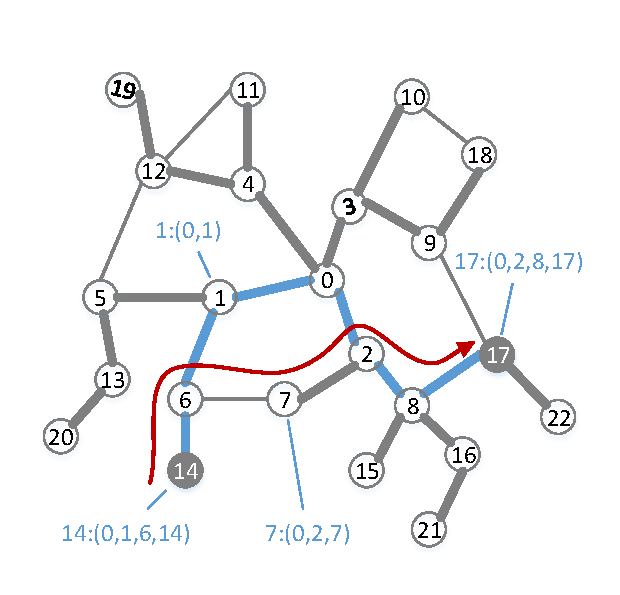
\epsfig{file=./figures/new_illustrate/ds_common.pdf,width=0.32\textwidth}\label{fig:DS:common}}
    \subfigure[Bi-directional Decentralized Search]{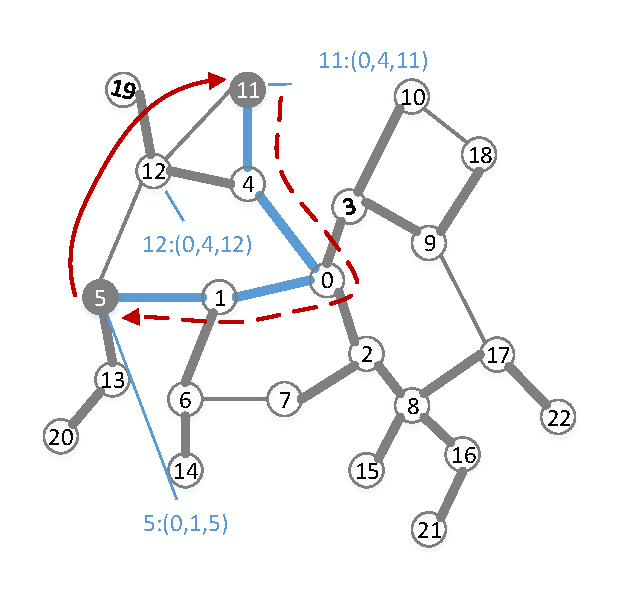
\epsfig{file=./figures/new_illustrate/ds_bidirectional.pdf,width=0.32\textwidth}\label{fig:DS:bidirectional}}
    \subfigure[Tie breaking strategy]{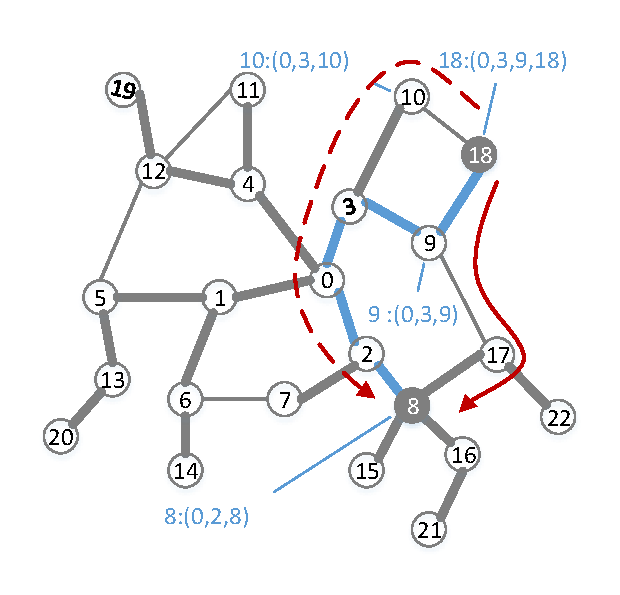
\epsfig{file=./figures/new_illustrate/ds_tie.pdf,width=0.32\textwidth}\label{fig:DS:tie}}
    \caption{Examples of decentralized search on indexed graph. Bold lines denote the indexed edges. Curved lines denoted paths being found, with arrows showing the direction. Dark vertices denote source and target vertex. Labels of vertices are shown in $vertex:label$ format.}
\end{figure*}

We propose to solve the point-to-point shortest path estimation problem using decentralized search with landmark based indexes. This section explains how to apply decentralized search on indexed graphs. Several aspects of the search including termination condition, bidirectional search and tie breaking strategy are discussed. 

\subsection{Index guided decentralized search}

To answer a shortest path query, decentralized search iteratively collect local distance information and visit vertex with least approximated distance to the target. More specifically, for a given pair of source $s$ and target vertex $t$ on an indexed graph, the search first sets the source vertex as the vertex to visit in the first step and appends it to the approximated path $\tilde{p}(s,t)$. At each step, suppose that the search is visiting vertex $u$, it traverse all the neighbor vertices of $u$. For each neighbor vertex $v_i$, the $d_{LCA}(v_i,t)$ is calculated. Then the search sets the neighbor vertex with smallest $d_{LCA}(v_i,t)$ as the vertex to visit in next step and appends $v_i$ to $\tilde{p}(s,t)$. 
 
Terminating when the search reaches the target vertex is a valid but not an ideal termination condition. Since shortest paths have optimal substructure, i.e. the path between any two vertices along a shortest path is also the shortest path of them. So the search can stop once it reach arbitrary vertex $u \in L(t)$ as the path $p_L(u,t) \subseteq L(t)$ is a shortest path from $u$ to $t$. Decentralized search cannot find a shorter path than $p_L(u,t)$. The detailed algorithm of decentralized search is depicted in Algorithm~\ref{alg:dec}.

\begin{algorithm}
    \caption{Decentralized search}
		\label{alg:dec}
    \begin{algorithmic}
        \Function{DecentralizedSearch}{$s$, $t$}
						\State $\tilde{p}(s,t) \gets \emptyset$
						\State $u \gets s$
						\State append $u$ to $\tilde{p}(s,t)$
						\While{$u \notin L(t)$}
								\State $d_{min} \gets \infty$
								\State $w \gets u$
								\For{each $v_i$ adjacent to $u$}
										\If{$d_{LCA}(v_i,t) < d_{min}$}
												\State $d_{min} \gets d_{LCA}(v_i,t)$
												\State $w \gets v_i$ 
										\EndIf
								\EndFor
								\State $u \gets w$
								\State append $u$ to $\tilde{p}(s,t)$
						\EndWhile
						\State $p_{remain} \gets p_L{u,t}$ excluding $u$
						\State append $p_{remain}$ to $\tilde{p}(s,t)$
						\State \Return $\tilde{p}(s,t)$
        \EndFunction
    \end{algorithmic}
\end{algorithm}

At each step, by examining neighbor vertices the search is able to explore a subset of the edges that is not indexed in the label of source and target vertex, which can potentially increase both accuracy and diversity of the path being found. For example in Fig.~\ref{fig:DS:common} from vertex $14$ to vertex $17$, decentralized search find a edge $(6, 7)$ as vertex $7$ has a LCA distance of $3$ which is shorter than LCA distance $5$ from vertex $1$ to $17$. 

\begin{theorem}
\label{theorem:max_step}
If the target vertex is reachable from the source, the decentralized search terminate in as much as $2{\sigma}_{max}$ steps, where ${\sigma}_{max}$ is the diameter of the graph. 
\end{theorem}
\begin{proof}[Sketch]
For an arbitrary source vertex $s$ and a reachable target vertex $t$, the following bound holds:
\[
    d_{LCA}(s,t) = d_G(s,LCA(s,t)) + d_G(LCA(s,t),t) \leq 2{\sigma}_{max}
\]
And at each step, suppose decentralized search is visiting vertex $u$ and $u \neq t$. Assume the tightest upper bound in equation~\ref{equ:upper} is achieved on shortest path tree $SPT_l$ rooted at landmark $l$. Let $v$ be the neighbor vertex of $u$ on path path $p_{LCA_l}(u,t)$. Since $SPT_l$ does not have cycle, $p_{LCA_l}(v,t) \in p_{LCA_l}(u,t)$. Therefore the following equation holds:
\[
		d_{LCA}(v,t) = |p_{LCA_l}(v,t)| = |p_{LCA_l}(u,t)| - 1 = d_{LCA}(u,t) - 1
\]
Since decentralized search always pick the neighbor with shortest LCA distance to the target, the LCA distance to the target at each step decreases at least by $1$. Therefore, the decentralized search terminates in at most $2{\sigma}_{max}$ steps. 
\end{proof}

The time complexity of Decentralized search depends on the max degree and the diameter of the graph. Decentralized search take at most $2{\sigma}_{max}$ steps to finish according to Theorem~\ref{theorem:max_step}. For each step, the search check at most ${\delta}_{max}$ neighbor vertices, where ${\delta}_{max}$ is the max vertex degree of the graph. For each neighbor, $k$ LCA computations are required, and time complexity for each LCA computation is $O(h)$\footnote{$O(h)$ is for simple online algorithm, off-line algorithms can achieve time complexity of $O(1)$.}, where $h$ is the height of the indexed shortest path tree and $h \leq {\sigma}_{max}$. So the worst case time complexity of decentralized search is $O(k{{\sigma}_{max}}^2{\delta}_{max})$.

The space complexity for decentralized search contains two parts, space complexity for offline index and space complexity for online query. The space required for offline index is $O(k{\sigma}_{max}n)$, where $n$ is number of vertices. For each query, $O(k{\sigma}_{max})$ space is required to store the labels of target vertex and the vertex that is being examined. $O(2{\sigma}_{max})$ space is required to store the approximated path. Combining them together, the online search space complexity of decentralized search is $O(k{\sigma}_{max})$. 

\subsection{Bi-directional search}

In this section, we show how to apply the idea of bidirectional search to decentralized search. In bidirectional decentralized search, the backward search starts at target vertex and is driven by the goal to reach the source vertex. The forward search and backward search may explore different search spaces due to the different start point and search goal. By exploring a different search space  the backward search may find a shorter approximated path. This, however, is quite different from the application of bidirectional search in BFS or A* search where the main focus is to reduce search space. 

An example of directional decentralized search is shown in Fig.~\ref{fig:DS:bidirectional}. Let $11$ be source and $5$ be target. The backward search can find a shorter path $p_{bwd} = (5, 12, 11)$ than the path $p_{fwd} = (11, 4, 0, 1, 5)$ found by the forward search. The backward search find a shorter path by exploring edge $(5, 12)$. However, this edge is invisible to forward search because when the search traversing vertex $4$, it prioritize $0$ than $12$ due to the former one has lower LDA distance to target vertex $5$. 

It is not guaranteed that the forward search and backward search will eventually meet at any vertex except the source and target vertex due to the different search space. As shown in our previous example, $p_{fwd} \cap p_{bwd} = (11, 5)$. Actually, in decentralized search, the forward search and backward search are mostly two independent search, that the only interaction of them is when combining the search results. Search results can be combined simply by picking the shorter path or finding short cuts connecting resulting paths. 

\subsection{Tie breaking strategy}

Ties happen frequently in decentralized search, especially when the number of landmarks is small. In the decentralized search, a tie means multiple neighbor vertices have same LCA distance to the target in a step. The reason a tie happens is that there is not sufficient information in the index that can separate neighbor vertices for a query. For example in Fig.~\ref{fig:DS:tie}, consider a search from $18$ to $8$. When traversing neighbors of vertex $18$, both vertex $10$ and $9$ have the same LCA distance to target vertex $8$, but their actual distances to vertex $8$ are different due to that short cut edge $(9, 17)$ is currently invisible to the decentralized search. 

The search space of the decentralized search can be increased by expanding the search onto each tie vertex. This increase both the performance, i.e. chances to find a shorter path and number of paths being found, and the cost of the search. 
By controlling the search space this way, decentralized search is able to achieve differentiate level of accuracy. 

Two extreme ways to deal with ties are either only visit one vertex or visit all vertices in the next step. The former one incurs least search cost and has the least possibility to find a shorter path, we refer to it as single branch decentralized search. The latter one requires most effort and can lead to the shortest path the decentralized search could possibly find, we refer to it as full branch decentralized search. 
